
\begin{frame}{SCS incomplete models: how to consider logic function?}
    \begin{textblock*}{6cm}(5mm, 22mm)
        \includegraphics[width=1.0\textwidth]{tripleWell_no_7c_Eevee.png}
    \end{textblock*}
    \begin{textblock*}{1cm}(65mm, 26.9mm)
        \tikz [line width=1mm]\draw [arrows = {-Stealth[length=10pt]}] (0,0) -- (1,1);
    \end{textblock*}

    \begin{textblock*}{45mm}(84mm, 16mm)
        \centering
        \includegraphics[width=1.0\textwidth]{./logicGatesSoloSignals/DW/vddGnd_illus.pdf}
    \end{textblock*}
    \begin{textblock*}{45mm}(84mm, 27mm)
        \centering
        \includegraphics[width=1.0\textwidth]{./logicGatesSoloSignals/DW/vepi_illus.pdf}
    \end{textblock*}

    \begin{textblock*}{1cm}(115.62mm, 38.65mm)
        \tikz [line width=1mm]\draw [arrows = {-Stealth[length=10pt]}] (0,0) -- (0.,-.8);
    \end{textblock*}

    \begin{textblock*}{1cm}(78mm, 16mm)
        
\begin{tikzpicture}
            \draw[decorate, decoration={brace, amplitude=10pt}, black, line width=1pt] (0, 0) -- (0.0, 2.0);
        \end{tikzpicture}
    \end{textblock*}

    \begin{textblock*}{1cm}(96mm, 50mm)
        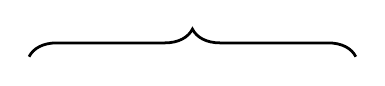
\begin{tikzpicture}
            \draw[decorate, decoration={brace, amplitude=10pt}, black, line width=1pt] (0, 0) -- (4.15, 0.0);
        \end{tikzpicture}
    \end{textblock*}

    \begin{textblock*}{5cm}(90mm, 55mm)
        
\includegraphics[width=1.0\textwidth]{ivx3New.pdf}
    \end{textblock*}
\end{frame}
